\chapter{FUNDAMENTAÇÃO TEÓRICA}
\label{FundamentacaoTeorica}

\section{Modelo de Banco de Dados Relacional}

O modelo relacional surgiu por volta dos anos de 1970, com base no modelo proposto por \citeonline{codd1970relational}. Através deste modelo, ``os dados são armazenados com um forte grau de independência, desacoplando a lógica, da representação dos dados'' \cite{davoudian2018survey}. Na representação relacional, os dados são normalizados e as diversas relações (tabelas) podem referenciar os dados contidos em outras tabelas.

Assim como explicado por \citeonline{date2004introduccao}, cada linha de uma tabela (tupla) deve representar a abstração de um objeto do sistema, sendo que cada célula é uma característica (atributo) do objeto representado. Cada tupla deve possuir pelo menos uma célula como identificador único (chave primária) que irá representar todos os dados contido na linha a qual ela está contida. A chave primária é um valor único para a tabela, geralmente representado com um tipo numérico. Tal chave pode ser armazenada em outras tabelas por meio do uso de chaves estrangeiras. Uma chave estrangeira é uma (ou mais de uma) chave primária de outra relação. Armazenar tal chave simboliza que os dados representados por ela estão contidos dentro da tabela.

Como exemplo, pode-se abstrair um sistema que precisa armazenar várias pessoas (na qual cada uma possui um nome e uma idade) e várias casas (que possui uma rua e número). A tabela \ref{tab: pessoa} apresenta como as pessoas podem estar representadas no banco de dados.

%%%%% REMOVIDO %%%%%
% Caso seja necessário armazenar os dados contidos em uma tupla de outra relação, basta, em alguma célula da tupla, armazenar uma chave estrangeira (chave primária de uma tupla de outra relação) de outra tabela. Ao armazenar como chave estrangeira a chave primária de outra tabela, é gerado um link lógico, simbolizando que todos os dados representados por esta chave estrangeira também estão contidos dentro desta mesma tupla.
%%%%% REMOVIDO %%%%%

%IMPORTANTE
%Os exemplos precisam ser referenciados

\begin{longtable}[]{@{}lll@{}}
\caption{Exemplo de relação de pessoas \label{tab: pessoa}}\tabularnewline
\toprule
Chave Primária & Nome & Idade \tabularnewline
\midrule
\endfirsthead
\toprule
Chave Primária & Nome & Idade\tabularnewline
\midrule
\endhead
1 & Emanuel & 21\tabularnewline
2 & Eduardo & 40\tabularnewline
\bottomrule
% \caption*{Fonte: O autor (2020)}
\end{longtable}

%%%%% REMOVIDO %%%%%
% \begin{table}[h]
%     \centering
%     \begin{tabular}{|c|c|c|}
%         \hline
%         \rowcolor[HTML]{FFAC71} 
%         \multicolumn{3}{|c|}{\cellcolor[HTML]{FFAC71}pessoa}                                                                                          \\ \hline
%         \rowcolor[HTML]{9698ED} 
%         {\color[HTML]{000000} \begin{tabular}[c]{@{}c@{}}Chave \\ Primária\end{tabular}} & {\color[HTML]{000000} Nome} & {\color[HTML]{000000} Idade} \\ \hline
%         1                                                                                & Emanuel                     & 21                           \\ \hline
%         2                                                                                & Eduardo                     & 40                           \\ \hline
%     \end{tabular}
%     \label{tab-ex1: pessoa}
%     \caption{Relação de pessoas}
% \end{table}

% \begin{table}[h]
%     \centering{
%         \begin{tabular}{|c|c|c|}
%             \hline
%             \rowcolor[HTML]{67FD9A} 
%             \multicolumn{3}{|c|}{\cellcolor[HTML]{67FD9A}casa}                                                                                            \\ \hline
%             \rowcolor[HTML]{9698ED} 
%             {\color[HTML]{000000} \begin{tabular}[c]{@{}c@{}}Chave \\ Primária\end{tabular}} & {\color[HTML]{000000} Rua} & {\color[HTML]{000000} Número} \\ \hline
%             10                                                                               & Rua Castelo Branco         & 1B                            \\ \hline
%             20                                                                               & Rua Pompel                 & 1089                          \\ \hline
%         \end{tabular}
%     }
% \end{table}
%%%%% REMOVIDO %%%%%

Continuando com o exemplo, naturalmente, no desenvolvimento de um sistema, as entidades se relacionam entre si. Neste caso, uma pessoa pode possuir várias casas, mas uma casa possui apenas uma pessoa como dono. Para representar essa relação, precisa-se definir quem será o dono da relação, ou seja, quem irá receber a chave primária da outra entidade através de uma chave estrangeira. Sempre deverá existir apenas  um dono da relação, ou seja, a chave estrangeira desta relação deverá estar em apenas uma tabela.
    
Como uma pessoa pode possuir várias casas, o dono da relação deve ser a casa, caso contrário a tupla de uma pessoa teria que ser duplicada (a menos que uma terceira tabela seja criada). Para representar as casas neste contexto, pode-se modelar os dados assim como demonstrado na tabela \ref{tab: casa}. Nela, pode-se observar que a pessoa Emanuel possui as duas casas armazenados no banco de dados, enquanto o Eduardo não possui nenhuma casa.

\begin{longtable}[]{@{}llll@{}}
\caption{Exemplo de relação de casas \label{tab: casa}}\tabularnewline
\toprule
Chave Primária & Rua & Número & Chave Estrangeira de Pessoa\tabularnewline
\midrule
\endfirsthead
\toprule
Chave Primária & Rua & Número & Chave Estrangeira de Pessoa\tabularnewline
\midrule
\endhead
10 & Rua Castelo Branco & 1B & 1\tabularnewline
20 & Rua Pompel & 1089 & 1\tabularnewline
\bottomrule
% \caption*{Fonte: O autor (2020)}
\end{longtable}

%%%%% REMOVIDO %%%%%
% \begin{table}[h]
%     \centering
%     \begin{tabular}{|c|c|c|c|}
%         \hline
%         \rowcolor[HTML]{67FD9A} 
%         \multicolumn{4}{|c|}{\cellcolor[HTML]{67FD9A}casa}                                                                                                                                                                        \\ \hline
%         \rowcolor[HTML]{9698ED} 
%         {\color[HTML]{000000} \begin{tabular}[c]{@{}c@{}}Chave \\ Primária\end{tabular}} & {\color[HTML]{000000} Rua} & {\color[HTML]{000000} Número} & \begin{tabular}[c]{@{}c@{}}Chave \\ Estrangeira \\ de pessoa\end{tabular} \\ \hline
%         10                                                                               & Rua Castelo Branco         & 1B                            & 1                                                                         \\ \hline
%         20                                                                               & Rua Pompel                 & 1089                          & 1                                                                         \\ \hline
%     \end{tabular}
%     \label{tab-ex1: casa}
%     \caption{Relação de casas}
% \end{table}
%%%%% REMOVIDO %%%%%

\subsection{Normalização}

O modelo relacional possui algumas regras que o desenvolvedor observa ao modelar as estruturas das relações de seu banco. Dentre estas regras estão contidas as regras de normalização. ``O objetivo da normalização é evitar os problemas de banco de dados, bem como eliminar a `mistura de assuntos' e as correspondentes redundâncias desnecessárias de dados'' \cite{machado2020banco}. Com a redução dessas ``redundâncias desnecessárias'', uma otimização da quantidade de dados é alcançada. \citeonline{machado2020banco} descreve 5 formas normais. Destas, apenas as 3 primeiras serão explicitadas a seguir, por terem impacto mais significante para os propósitos deste trabalho.

%%%%% DÚVIDAS %%%%%
% As regras de nornalização realmente devem ser seguidas em todas as circunstâncias?
% R - creio que são questões organizacionais e que facilitam as consultas
%%%%% DÚVIDAS %%%%%

%%%%% PENDÊNCIAS %%%%%
% Justificar através de citações o parâgrafo anterior
%%%%% PENDÊNCIAS %%%%%

\subsubsection{Primeira Forma Normal}
    
Como visto anteriormente, uma tupla representa um objeto da entidade representada pela relação a qual a tupla pertence. Tendo esse princípio como base, como é possível representar a situação de uma casa possuir vários donos e ao mesmo tempo uma pessoa possuir várias casas?
    
O princípio da primeira forma normal define que nunca deve-se duplicar colunas em várias linhas, garantindo que duas ou mais tuplas nunca representem o mesmo objeto. Para manter este princípio e ainda realizar um relacionamento de muitos para muitos (uma pessoa tem muitas casas e uma casa tem muitas pessoas), torna-se necessário a criação de uma tabela auxiliar para representar o relacionamento de pessoa com casa. A tabela \ref{tab: relacionamento-pessoa-casa} exemplifica a criação de uma tabela auxiliar, na qual a pessoa ``Emanuel'' possui as duas casas e o ``Eduardo'' possui a casa de número 1B.

\begin{longtable}[]{@{}lll@{}}
\caption{Exemplo de tabela auxiliar \label{tab: relacionamento-pessoa-casa}}\tabularnewline
\toprule
Chave Primária & Chave Estrangeira de Pessoa & Chave Estrangeira de Casa\tabularnewline
\midrule
\endfirsthead
\toprule
Chave Primária & Chave Estrangeira de Pessoa & Chave Estrangeira de Casa\tabularnewline
\midrule
\endhead
100 & 1 & 10\tabularnewline
200 & 1 & 20\tabularnewline
300 & 2 & 10\tabularnewline
\bottomrule
% \caption*{Fonte: O autor (2020)}
\end{longtable}

%%%%% REMOVIDO %%%%%
% \begin{longtable}[]{@{}llcl@{}}
% \caption{Exemplo de relação de pessoas \label{tab-ex2: pessoa}}\tabularnewline
% \toprule
% Chave Primária & Nome & Idade \tabularnewline
% \midrule
% \endfirsthead
% \toprule
% Chave Primária & Nome & Idade\tabularnewline
% \midrule
% \endhead
% 1 & Emanuel & 21\tabularnewline
% 2 & Eduardo & 40\tabularnewline
% \bottomrule
% \caption*{Fonte: O autor (2020)}
% \end{longtable}

% \begin{longtable}[]{@{}llcl@{}}
% \caption{Exemplo de relação de casas \label{tab-ex2: casa}}\tabularnewline
% \toprule
% Chave Primária & Rua & Número & Chave Estrangeira de pessoa\tabularnewline
% \midrule
% \endfirsthead
% \toprule
% Chave Primária & Rua & Número & Chave Estrangeira de pessoa\tabularnewline
% \midrule
% \endhead
% 10 & Rua Castelo Branco & 1B & 1\tabularnewline
% 20 & Rua Pompel & 1089 & 1\tabularnewline
% \bottomrule
% \caption*{Fonte: O autor (2020)}
% \end{longtable}

% \begin{table}[h]
%         \centering
%         \begin{tabular}{|c|c|c|}
%             \hline
%             \rowcolor[HTML]{FFAC71} 
%             \multicolumn{3}{|c|}{\cellcolor[HTML]{FFAC71}pessoa}                                                                                          \\ \hline
%             \rowcolor[HTML]{9698ED} 
%             {\color[HTML]{000000} \begin{tabular}[c]{@{}c@{}}Chave \\ Primária\end{tabular}} & {\color[HTML]{000000} Nome} & {\color[HTML]{000000} Idade} \\ \hline
%             1                                                                                & Emanuel                     & 21                           \\ \hline
%             2                                                                                & Eduardo                     & 40                           \\ \hline
%         \end{tabular}
% \end{table}
    
% \begin{table}[h]
%         \centering
%         \begin{tabular}{|c|c|c|}
%             \hline
%             \rowcolor[HTML]{FCFF2F} 
%             \multicolumn{3}{|c|}{\cellcolor[HTML]{FCFF2F}Relacionamentopessoacasa}                                                                                                                                                                                                                                   \\ \hline
%             \rowcolor[HTML]{9698ED} 
%             {\color[HTML]{000000} \begin{tabular}[c]{@{}c@{}}Chave \\ Primária do\\ Relacionamento\end{tabular}} & {\color[HTML]{000000} \begin{tabular}[c]{@{}c@{}}Chave \\ Estrangeira \\ de pessoa\end{tabular}} & {\color[HTML]{000000} \begin{tabular}[c]{@{}c@{}}Chave \\ Estrangeira \\ de casa\end{tabular}} \\ \hline
%             100                                                                                                    & 1                                                                                                & 10                                                                                             \\ \hline
%             200                                                                                                    & 1                                                                                                & 20                                                                                             \\ \hline
%             300                                                                                                    & 2                                                                                                & 10                                                                                             \\ \hline
%         \end{tabular}
% \end{table}
    
% \begin{table}[h]
%         \centering
%         \begin{tabular}{|c|c|c|}
%             \hline
%             \rowcolor[HTML]{67FD9A} 
%             \multicolumn{3}{|c|}{\cellcolor[HTML]{67FD9A}casa}                                                                                            \\ \hline
%             \rowcolor[HTML]{9698ED} 
%             {\color[HTML]{000000} \begin{tabular}[c]{@{}c@{}}Chave \\ Primária\end{tabular}} & {\color[HTML]{000000} Rua} & {\color[HTML]{000000} Número} \\ \hline
%             10                                                                               & Rua Castelo Branco         & 1B                            \\ \hline
%             20                                                                               & Rua Pompel                 & 1089                          \\ \hline
%         \end{tabular}
% \end{table}
%%%%% REMOVIDO %%%%%
    
\subsubsection{Segunda Forma Normal}
    
A segunda forma normal especifica que todos os dados de uma tupla devem ser representados por toda a sua chave primária e jamais por apenas parte dela. Como exemplo disto pode-se afirmar que uma casa jamais poderia ser armazenado dentro da mesma tupla de uma pessoa, mesmo em um relacionamento um para um (Uma pessoa para uma casa e uma casa para uma pessoa). Isto ocorre pois os dados de uma casa são independentes dos dados de uma pessoa e a chave primária de uma pessoa não poderia representar também os dados de uma casa.
    
Uma chave primária também pode ser composta por várias células, mas todos os dados da tupla devem depender de todas as células da chave primária. Caso exista algum dado que dependa apenas de parte da chave primária, uma nova tabela deve ser criada. Uma tabela somente está na segunda forma normal se também estiver na primeira forma normal.
    
\subsubsection{Terceira Forma Normal}
    
Continuando o exemplo, pode-se imaginar que devem existir atributos no relacionamento entre pessoa e casa, indicando o valor mensal que a pessoa deve pagar como aluguel pela casa, a quantidade de meses a pagar o aluguel e o total a pagar até o fim do contrato. Para isso, poderíamos adicionar tais atributos na tabela de relacionamento de pessoa com casa, assim como descrito na tabela \ref{tab: atributos-relacionamento}. Nesta, a pessoa de nome ``Emanuel'' paga 200 reais pela casa de número 1B com contrato válido por 12 meses e paga 400 reais pela casa de número 1089 com contrato válido por 24 meses. O Eduardo paga 300 reais pela casa de número 1B com contrato válido por 8 meses.

\begin{longtable}[]{@{}llllll@{}}
\caption{Exemplo Atributos no Relacionamento \label{tab: atributos-relacionamento}}\tabularnewline
\toprule
Chave Primária & Pessoa & Casa & Valor Mensal & Quantidade de Meses & Total\tabularnewline
\midrule
\endfirsthead
\toprule
Chave Primária & Pessoa & Casa & Valor Mensal & Quantidade de Meses & Total\tabularnewline
\midrule
\endhead
100 & 1 & 10 & 200 & 12 & 2400\tabularnewline
200 & 1 & 20 & 400 & 24 & 9600\tabularnewline
300 & 2 & 10 & 300 & 8  & 2400\tabularnewline
\bottomrule
% \caption*{Fonte: O autor (2020)}
\end{longtable}

%%%%% REMOVIDO %%%%%
% \begin{table}[h]
%     \centering
%     \begin{tabular}{|c|c|c|c|c|c|}
%         \hline
%         \rowcolor[HTML]{FCFF2F} 
%         \multicolumn{6}{|c|}{\cellcolor[HTML]{FCFF2F}Relacionamentopessoacasa}                                                                                                                                                                                                                                                                                                                                                                                                                      \\ \hline
%         \rowcolor[HTML]{9698ED} 
%         {\color[HTML]{000000} \begin{tabular}[c]{@{}c@{}}Chave \\ Primária do\\ Relacionamento\end{tabular}} & {\color[HTML]{000000} \begin{tabular}[c]{@{}c@{}}Chave \\ Estrangeira \\ de pessoa\end{tabular}} & {\color[HTML]{000000} \begin{tabular}[c]{@{}c@{}}Chave \\ Estrangeira \\ de casa\end{tabular}} & \begin{tabular}[c]{@{}c@{}}Valor\\ Mensal\end{tabular} & \begin{tabular}[c]{@{}c@{}}Quantidade\\ de Meses\end{tabular} & \begin{tabular}[c]{@{}c@{}}Total a\\ Pagar\end{tabular} \\ \hline
%         100                                                                                                    & 1                                                                                                & 10                                                                                             & 200                                                    & 12                                                            & 2400                                                    \\ \hline
%         200                                                                                                    & 1                                                                                                & 20                                                                                             & 400                                                    & 24                                                            & 9600                                                    \\ \hline
%         300                                                                                                    & 2                                                                                                & 10                                                                                             & 300                                                    & 8                                                             & 2400                                                    \\ \hline
%     \end{tabular}
% \end{table}
%%%%% REMOVIDO %%%%%
    
Para este caso, a relação \ref{tab: atributos-relacionamento} não está na terceira forma normal, pois o atributo \textit{Total} é dependente do \textit{Valor Mensal} e da \textit{Quantidade de Meses}. O \textit{Total} pode ser obtido através de uma busca no banco de dados, realizando uma simples multiplicação do \textit{Valor Mensal} e da \textit{Quantidade de Meses}. Para que esta relação fique de acordo com a Terceira Forma Normal é necessário remover a última coluna, assim como apresentado na tabela \ref{tab: total-a-pagar-removido}.
    
\begin{longtable}[]{@{}lllll@{}}
\caption{``Total'' Removido \label{tab: total-a-pagar-removido}}\tabularnewline
\toprule
Chave Primária & Pessoa & Casa & Valor Mensal & Quantidade de Meses\tabularnewline
\midrule
\endfirsthead
\toprule
Chave Primária & Pessoa & Casa & Valor Mensal & Quantidade de Meses\tabularnewline
\midrule
\endhead
100 & 1 & 10 & 200 & 12\tabularnewline
200 & 1 & 20 & 400 & 24\tabularnewline
300 & 2 & 10 & 300 & 8\tabularnewline
\bottomrule
% \caption*{Fonte: O autor (2020)}
\end{longtable}

%%%%% REMOVIDO %%%%%
% \begin{table}[h]
%     \centering
%     \begin{tabular}{|c|c|c|c|c|}
%         \hline
%         \rowcolor[HTML]{FCFF2F} 
%         \multicolumn{5}{|c|}{\cellcolor[HTML]{FCFF2F}Relacionamentopessoacasa}                                                                                                                                                                                                                                                                                                                                                            \\ \hline
%         \rowcolor[HTML]{9698ED} 
%         {\color[HTML]{000000} \begin{tabular}[c]{@{}c@{}}Chave \\ Primária do\\ Relacionamento\end{tabular}} & {\color[HTML]{000000} \begin{tabular}[c]{@{}c@{}}Chave \\ Estrangeira \\ de pessoa\end{tabular}} & {\color[HTML]{000000} \begin{tabular}[c]{@{}c@{}}Chave \\ Estrangeira \\ de casa\end{tabular}} & \begin{tabular}[c]{@{}c@{}}Valor\\ Mensal\end{tabular} & \begin{tabular}[c]{@{}c@{}}Quantidade\\ de Meses\end{tabular} \\ \hline
%         1                                                                                                    & 1                                                                                                & 10                                                                                             & 200                                                    & 12                                                            \\ \hline
%         2                                                                                                    & 1                                                                                                & 20                                                                                             & 400                                                    & 24                                                            \\ \hline
%         3                                                                                                    & 2                                                                                                & 10                                                                                             & 300                                                    & 8                                                             \\ \hline
%     \end{tabular}
% \end{table}
%%%%% REMOVIDO %%%%%
    
A terceira forma normal especifica que não deve existir uma célula que dependa de outras células. Cada valor deverá ser o mais independente possível dos outros valores. Para que uma relação esteja na terceira forma normal, também torna-se necessário que esteja na segunda forma normal.

\subsection{Junção de Tabelas\label{subsection: juncao-tabelas}}
    
Assim como descrito por \citeonline{machado2020banco}, existem situações onde as tabelas precisam ser unidas em uma única tabela, para que os dados contidos em diversas relações, que são necessários à consulta formulada, possam ser acessados. Como exemplo disto, pode-se unir as tabelas \ref{tab: pessoa}, \ref{tab: casa} e \ref{tab: total-a-pagar-removido}, para a pessoa de nome \textit{Emanuel}. No exemplo \ref{lst: uniao-tabelas-sql} encontra-se uma codificação SQL para a união de tabelas para o contexto apresentado. A seguir, na tabela \ref{tab: juncao-de-tabelas-para-emanuel} apresenta-se o resultado de tal codificação.

% \newpage

\begin{lstlisting}[language=SQL, caption={União de Tabelas com SQL\label{lst: uniao-tabelas-sql}}]
    SELECT p.id as Pessoa, p.nome as Nome, p.idade as Idade, rpc.valor_mensal as ValorMensal, rpc.quantidade_meses as Meses, c.id as Casa, c.rua as Rua, c.numero as Numero
    FROM pessoa p JOIN
        Relacionamentopessoacasa rpc ON p.id = rpc.pessoa_id JOIN
        casa c ON rpc.casa_id = c.id
    WHERE p.nome = "Emanuel"
\end{lstlisting}

\newpage

\begin{longtable}[]{@{}llllllll@{}}
\caption{Junção de Tabelas Para Emanuel \label{tab: juncao-de-tabelas-para-emanuel}}\tabularnewline
\toprule
\footnotesize{Pessoa} & \footnotesize{Nome} & \footnotesize{Idade} & \footnotesize{ValorMensal} & \footnotesize{Meses} & \footnotesize{Casa} & \footnotesize{Rua} & \footnotesize{Numero}\tabularnewline
\midrule
\endfirsthead
\toprule
\footnotesize{Pessoa} & \footnotesize{Nome} & \footnotesize{Idade} & \footnotesize{ValorMensal} & \footnotesize{Meses} & \footnotesize{Casa} & \footnotesize{Rua} & \footnotesize{Numero}\tabularnewline
\midrule
\endhead
\footnotesize{1} & \footnotesize{Emanuel} & \footnotesize{21} & \footnotesize{200} & \footnotesize{12} & \footnotesize{10} & \footnotesize{Rua Castelo Branco} & \footnotesize{1B}\tabularnewline
\footnotesize{1} & \footnotesize{Emanuel} & \footnotesize{21} & \footnotesize{400} & \footnotesize{24} & \footnotesize{20} & \footnotesize{Rua Pompel} & \footnotesize{1089}\tabularnewline
\bottomrule
% \caption*{Fonte: O autor (2020)}
\end{longtable}

%%%%% REMOVIDO %%%%%
%     \begin{table}[h]
%         \centering
%         \resizebox{\textwidth}{!}{%
%             \begin{tabular}{|c|c|c|c|c|c|c|c|c|c|c|}
%                 \hline
%                 \rowcolor[HTML]{38FFF8} 
%                 \multicolumn{11}{|c|}{\cellcolor[HTML]{38FFF8}Junção das Três Tabelas}                                                                                                                                                                                                                                                                                                                                                                                                                                                                                                                                                        \\ \hline
%                 \rowcolor[HTML]{9698ED} 
%                 \begin{tabular}[c]{@{}c@{}}Chave\\ Primária\\ de pessoa\end{tabular} & Nome    & Idade & {\color[HTML]{000000} \begin{tabular}[c]{@{}c@{}}Chave \\ Primária do\\ Relacionamento\end{tabular}} & {\color[HTML]{000000} \begin{tabular}[c]{@{}c@{}}Chave \\ Estrangeira \\ de pessoa\end{tabular}} & {\color[HTML]{000000} \begin{tabular}[c]{@{}c@{}}Chave \\ Estrangeira \\ de casa\end{tabular}} & \begin{tabular}[c]{@{}c@{}}Valor\\ Mensal\end{tabular} & \begin{tabular}[c]{@{}c@{}}Quantidade\\ de Meses\end{tabular} & \begin{tabular}[c]{@{}c@{}}Chave\\ Primária\\ de casa\end{tabular} & Rua                & Número \\ \hline
%                 1                                                                    & Emanuel & 21    & 100                                                                                                    & 1                                                                                                & 10                                                                                             & 200                                                    & 12                                                            & 10                                                                 & Rua Castelo Branco & 1B     \\ \hline
%                 1                                                                    & Emanuel & 21    & 200                                                                                                    & 1                                                                                                & 20                                                                                             & 400                                                    & 24                                                             & 20                                                                 & Rua Pompel & 1089     \\ \hline
%             \end{tabular}%
%         }
%     \end{table}
    
% Neste caso, algumas colunas do relacionamento de pessoa com casa são desnecessárias e no comando de junção das tabelas pode-se omití-las. Neste caso a tabela de junção seria algo como:
    
%     \begin{table}[h]
%         \centering
%         \resizebox{\textwidth}{!}{%
%             \begin{tabular}{|c|c|c|c|c|c|c|c|}
%                 \hline
%                 \rowcolor[HTML]{38FFF8} 
%                 \multicolumn{8}{|c|}{\cellcolor[HTML]{38FFF8}Junção das Três Tabelas}                                                                                                                                                                                                                                              \\ \hline
%                 \rowcolor[HTML]{9698ED} 
%                 \begin{tabular}[c]{@{}c@{}}Chave\\ Primária\\ de pessoa\end{tabular} & Nome    & Idade & \begin{tabular}[c]{@{}c@{}}Valor\\ Mensal\end{tabular} & \begin{tabular}[c]{@{}c@{}}Quantidade\\ de Meses\end{tabular} & \begin{tabular}[c]{@{}c@{}}Chave\\ Primária\\ de casa\end{tabular} & Rua                & Número \\ \hline
%                 1                                                                    & Emanuel & 21    & 200                                                    & 12                                                            & 10                                                                 & Rua Castelo Branco & 1B     \\ \hline
%                 1                                                                    & Emanuel & 21    & 400                                                    & 24                                                             & 20                                                                 & Rua Pompel & 1089     \\ \hline
%             \end{tabular}%
%         }
%     \end{table}
%%%%% REMOVIDO %%%%%

Quando há a separação dos dados, a atualização destes tendem a garantir uma maior consistência, além de tentar garantir que os valores precisarão ser atualizados em um único local. Mas em buscas no banco de dados, as junções de tabelas são, muitas vezes, inevitáveis.

%%%%% PENDÊNCIAS %%%%%
% Referenciar trabalhos que demonstrem que a separação dos dados tem o proposito apresentado no parágrafo anterior
% R - nesse caso também não precisa referenciar, pois vc ta fazendo uma constatação de quem programa
%%%%% PENDÊNCIAS %%%%%
    
Em um sistema complexo, com uma grande quantidade de dados e relações, cada tabela poderá conter milhares ou até milhões de linhas. Uma operação de junção, envolvendo muitos dados, pode ser lento demais para os requisitos da aplicação. Existem algumas técnicas e estratégias para deixar essas consultas mais rápidas, como, por exemplo, o uso de índices. Mas mesmo com essas estratégias, haverá aplicações na qual a exigência de alta performance, escalabilidade, disponibilidade e consistência tornará inviável ou altamente caro escalar uma aplicação utilizando o modelo relacional.

%%%%% PENDÊNCIAS %%%%%
% Referenciar na literatura tais técnicas e estratégias
% R - Nesse caso se encontrar algum trabalho seria bom, mas ainda assim não é obrigatório.
%%%%% PENDÊNCIAS %%%%%

\subsection{Vantagens do Modelo relacional}
    
\begin{itemize}
    \item O modelo relacional já está bem solidificado no mercado, possuindo várias ferramentas e \textit{frameworks} para facilitar o desenvolvimento dos mais diversos tipos de aplicações;
        
    \item Pelo fato do modelo relacional forçar a separação e normalização dos dados, torna-se mais difícil que erros humanos ou de desenvolvimento venham a fazer os dados perderem sua consistência;
        
%    \item A normalização dos dados proporciona que os dados possam ser
%         inseridos/atualizados sem que o usuário/desenvolvedor tenha a responsabilidade de 
%         fazer diversas verificações físicas/lógicas na própria estrutura de armazenamento de
%         dados;
        
%    \item Uma modelagem de dados mal planejada possui menos chances de causar grandes
%         danos a consistência dos dados por causa da normalização;
        
    \item A normalização, por causa de seu princípio de não repetir dados em várias tabelas, tende a diminuir o espaço necessário para armazenar os dados, além de a atualização de registros, no geral, ocorrer em apenas um local.
\end{itemize}
    
\subsection{Desvantagens do Modelo relacional}

%%%%% DÚVIDAS %%%%%
% Precisa justificar tais desvantagens por meio de citações às referências bibliográficas?
%%%%% DÚVIDAS %%%%%
    
\begin{itemize}
    \item Os recursos de modelagem são muito limitados;
        
    \item A construção de objetos por meio de operações de junção, muitas vezes, são caras;
        
    \item O modelo relacional revelou deficiências no armazenamento e consulta de um grande volume de dados;
        
    \item Diversas aplicações com altos requisitos de escalabilidade, disponibilidade e consistência se tornam caras ou inviáveis no modelo relacional;
        
    \item As aplicações precisam se adaptar ao modelo relacional. Mesmo que uma aplicação possa ter uma parte dos dados não normalizados, sem prejudicar a consistência (por causa de alguma regra de negócio), o modelo relacional exige a normalização em vários casos, para um bom funcionamento das consultas.
\end{itemize}

\section{Modelo de Banco de Dados NoSQL com \textit{MongoDB}}

%%%%% REMOVIDO %%%%%
% Desde o início dos anos 2000, os avanços na tecnologia web, resultaram na explosão repentina de dados estruturados, semi-estruturados e não estruturados por aplicativos de escopo global. Tais aplicações geralmente exigem uma escalabilidade horizontal, adaptar-se às enormes quantidades de dados e à taxa crescente de processamento de consultas \citeonline{davoudian2018survey}.

% A alta disponibilidade, a baixa tolerância a falhas para responder aos clientes, confiabilidade de transações, o suporte a dados altamente consistentes e a manutenção de \textit{schemas} de banco de dados com baixo custo de evolução do sistema são requisitos que se tornam muitos difíceis ou inatingíveis nos sistemas tradicionais de banco de dados relacional \citeonline{davoudian2018survey}.Além desse motivo, a ampliação de sistemas exige uma movimentação de servidores autônomos com hardware aprimorados, sendo um processo caro e causa uma indisponibilidade significativa a cada movimentação. Sistemas baseados em modelos Relacionais exigem uma complexidade e sobrecarga maiores para se juntar dados distribuídos normalizados \citeonline{davoudian2018survey}.

% Os modelos de banco de dados NoSQL tornaram-se uma tendência emergente de armazenamento de dados não relacional, que visam satisfazer os requisitos de alta disponibilidade e escalabilidade de aplicações de âmbito global \citeonline{davoudian2018survey}.
%%%%% REMOVIDO %%%%%

Assim como descrito por \citeonline{davoudian2018survey}, o uso do modelo de banco de dados relacional tornam os requisitos de alta disponibilidade, baixa tolerância a falhas para responder aos clientes, confiabilidade das transações, suporte a dados altamente consistentes e manutenção de \textit{schemas} com baixo custo de evolução, muito difíceis ou inatingíveis. Além dos problemas apresentados, \citeonline{davoudian2018survey} ainda descrevem que os sistemas baseados em modelos relacionais trazem uma maior complexidade e sobrecarga para unir dados distribuídos normalizados. Por causa de tais problemas, houve uma demanda por um novo modelo de banco de dados. O modelo que tornou-se uma tendência emergente para o armazenamento de dados não relacional é o NoSQL, que foi projetado para satisfazer os requisitos de alta disponibilidade e escalabilidade de aplicações de âmbito global.
    
Um modelo de Banco de Dados NoSQL é caracterizado pela utilização de um modelo não relacional ou parcialmente relacional para o armazenamento de dados. Vários modelos NoSQL foram criados visando os princípios acima descritos. Para os propósitos deste trabalho, esta seção utiliza como base a descrição e utilização de modelos de banco de dados Baseado em Documento, sendo exemplificado pela descrição e uso do banco de dados \textit{MongoDB}.

Enquanto que no modelo relacional o armazenamento ocorre em uma tabela, no MongoDB o armazenamento ocorre em uma coleção de documentos, sendo cada documento a representação de um objeto do sistema. Cada banco de dados NoSQL baseado em Documento terá a sua própria estrutura de documento. No caso específico do \textit{MongoDB}, os documentos são escritos de maneira estruturada, seguindo uma variação do formato JSON (\textit{JavaScript Object Notation}). Tal variação possui o nome de BSON (\textit{Binary} JSON).

\subsection{O Formato JSON}
    
Assim como descrito por \citeonline{boaglio2015mongodb}, O JSON é um formato de representação de dados na qual um objeto possui uma lista de atributos. Um atributo é o nome de uma característica pertencente ao objeto na qual o JSON representa. Cada atributo possui um valor associado a ele. Tal valor pode ser \textit{null} (valor vazio), \textit{true} (verdadeiro), \textit{false} (falso), textual (entre aspas), numérico (sem aspas), pode ser um outro JSON (definido entre chaves) e pode ser uma lista de qualquer um dos tipos definidos anteriormente (entre colchetes separados por vírgula).

No exemplo \ref{lst: json-pessoas} é apresentado uma representação de uma lista de pessoas com suas respectivas casas. Nele, observa-se que a representação de um objeto é dada entre chaves (\textit{\{\}}) e, dentro dessas chaves, são definidos os nomes dos atributos do objeto (entre aspas) e, após os dois pontos (\textit{:}), é definido o valor para aquele atributo. Quando se deseja que o valor seja uma lista de elementos, envolve-se todos os elemento da lista entre colchetes (\textit{[]}) e cada elemento é separado por vírgula (\textit{,}).

% \newpage

\begin{lstlisting}[language=json, caption={JSON Representando Várias Pessoas Com Suas casas\label{lst: json-pessoas}}]
[{
    "nome": "Emanuel",
    "idade": 21,
    "casas": [
        {
            "rua": "Rua Castelo Branco",
            "numero": "1B",
            "valorMensal": 200,
            "quantidadeMeses": 12
        },
        {
            "rua": "Rua Pompel",
            "numero": 1089,
            "valorMensal": 400,
            "quantidadeMeses": 24
        }
    ]
},{
    "nome": "Eduardo",
    "idade": 40,
    "casas": {
        "rua": "Rua Pompel",
        "numero": "1089",
        "valorMensal": 300,
        "quantidadeMeses": 8
    }
}]
\end{lstlisting}
    
No exemplo \ref{lst: json-pessoas}, está sendo representado uma lista de objetos. Para a representação desta lista, as pessoas (JSON) são envolvidas entre colchetes. Caso seja desejado representar apenas uma pessoa (ao invés de uma lista), bastaria remover os colchetes mais externos e deixar apenas um JSON na raiz do documento. Observa-se que a pessoa com o nome \textit{Eduardo} possui apenas uma casa, e por este motivo o valor do atributo \textit{casa} pode ser representado como um JSON, mas também seria possível representar como uma lista de apenas uma casa. Para isto, bastaria, apenas, envolver as chaves (\textit{\{\}}) em colchetes (\textit{[]}), assim como ocorre para a pessoa \textit{Emanuel}.

\subsection{Coleções de Documentos no \textit{MongoDB}}
    
O formato de documento utilizado pelo \textit{MongoDB} é uma variação do JSON: o BSON (\textit{Binary JSON}). O BSON é uma extensão do JSON, suportando novos tipos de dados. De acordo com \citeonline{boaglio2015mongodb}, os novos tipos de dados suportados são:

\begin{enumerate}
    \item \textit{MinKey}, \textit{MaxKey}, \textit{Timestamp} --- Tipos utilizados internamente no \textit{MongoDB}

    \item \textit{BinData} --- \textit{Array} de \textit{bytes} para dados binários

    \item \textit{ObjectId} --- Identificador único de um registro do \textit{MongoDB}

    \item Date --- Representação de data
    
    \item Expressões Regulares
\end{enumerate}

Enquanto que no modelo relacional uma tabela representa uma coleção de objetos no sistema, no \textit{MongoDB}, esta representação é feita por uma coleção de documentos. Da mesma forma, enquanto uma tupla de uma tabela representa, no modelo relacional, um objeto, no \textit{MongoDB}, esta representação é feita por um documento, que possui, em seu interior, um BSON (não uma lista, mas apenas um único BSON).
    
Seguindo esta abordagem, para, por exemplo, armazenarmos várias pessoas no banco, precisa ser criado uma coleção que irá armazenar vários documentos, sendo cada documento uma representação de uma pessoa diferente. Cada pessoa terá um identificador único para a coleção (\textit{\_id}), que irá  representar o documento. Através deste identificador, pode-se fazer relações entre BJSONs diferentes. Tal identificador pode ser de qualquer tipo, porém, existe um tipo de dados chamado de \textit{ObjectId} criado especificamente para ser usado como um identificador único. O valor do \textit{ObjectId} pode ser explicitamente definido pelo usuário. Caso o usuário não o forneça, o \textit{MongoDB} irá defini-lo de forma automática. De acordo com \citeonline{boaglio2015mongodb}, o valor gerado não é sequencial, pois ele é criado baseado no \textit{timestamp}, o ID da máquina, o ID do processo e um contador local.

%%%%% REMOVIDO %%%%%
% A seguir é listado algumas vantagens do uso do \textit{ObjectId}:

% \begin{itemize}
%     \item O \textit{ObjectId} é formado por 12 bytes, sendo os quatro primeiros refletidos no \textit{timestamp} de quando o documento foi criado e possui uma \hl{probabilidade muito alta} de ser único. Por causa disto, é possível obter a data de criação de um documento pelo identificador
    
%     \item Odenar pelo \textit{\_id} com o tipo \textit{ObjectId} é equivalente a ordenar os documentos pela data de criação (para os documentos criados no mesmo segundo não é garantido nenhuma ordem)
    
%     \item O campo \textit{\_id} é automaticamente criado caso não seja informado
% \end{itemize}
%%%%% REMOVIDO %%%%%

%%%%%
% Qual a probabilidade do ObjectId ser único? Usar o termo "muito" pode ser inadequado
%%%%%

No exemplo \ref{lst: bjson-de-emanuel} está sendo exemplificado um BSON que poderia ser armazenado em um documento do \textit{MongoDB}, para representar a pessoa de nome ``Emanuel''. Para ilustrar a flexibilidade do valor do \textit{\_id}, o identificador das entidades serão armazenados por meio de um valor numérico, porém os identificadores dos BSON ``internos'' serão definidos como um \textit{ObjectId}. Esta escolha foi tomada, apenas, para facilitar a visualização dos exemplos, mas em um sistema, o \textit{\_id} poderia assumir qualquer tipo de dado.

\begin{lstlisting}[language=json, caption={BJSON da pessoa \textit{Emanuel}\label{lst: bjson-de-emanuel}}]
{
    "_id": 1,
    "nome": "Emanuel",
    "idade": 21,
    "casas": [
        {
            _id: ObjectId("5e66c969d5d7cc24c0850854"),
            "rua": "Rua Castelo Branco",
            "numero": "1B",
            "valorMensal": 200,
            "quantidadeMeses": 12
        },
        {
            _id: ObjectId("5e66c9740efbf528b05a7537"),
            "rua": "Rua Pompel",
            "numero": 1089,
            "valorMensal": 400,
            "quantidadeMeses": 24
        }
    ]
}
\end{lstlisting}

O identificador (\textit{\_id}) deve existir pelo menos no BSON principal (neste caso, aquele que representa uma pessoa). O BSON que representa uma casa não necessariamente precisa de um identificador, mas, para este exemplo, optou-se por gerar um. O identificador do BSON de uma casa não é o identificador de outro documento, pois, neste exemplo os dados estão desnormalizados e, por enquanto, para o exemplo apresentado, não existe outra coleção além da coleção de pessoa.

\subsection{Desnormalização}

Assim como descrito por \citeonline{date2004introduccao}, a desnormalização é o agrupamento de dados (que estariam separados em diferentes coleções, pelas formas normais) em uma única coleção. É um armazenamento, gerando redundância, sem a preocupação de seguir as formas normais, para unir dados relevantes em um único local. No exemplo apresentado, a coleção de casa não existe e as casas estão armazenadas dentro do mesmo BSON na qual uma pessoa é armazenada. Tal estrutura desobedece a segunda forma normal, pois o identificador do documento (\textit{\_id}) identifica uma pessoa, não podendo, portanto, identificar os dados das casas que estão presente no próprio documento.
    
Uma das principais vantagens da desnormalização é que, em vários casos, não existe a necessidade de realizar junção de vários documentos, podendo ter um ganho substancial de performance. No exemplo apresentado do modelo relacional (\ref{lst: uniao-tabelas-sql}), foi necessário realizar buscas e uniões de tabelas para obter uma relação contendo um balanço da lista total de casas da pessoa com nome \textit{Emanuel}. No \textit{MongoDB}, caso desejemos realizar a mesma pesquisa para a pessoa \textit{Emanuel}, obtendo a lista de casas que ela possui, não haveria a necessidade de juntar quaisquer documentos. Para isto, bastaria, apenas, buscar o BJSON da pessoa a qual se deseja buscar e retornar o documento, tal qual como foi armazenado. No modelo relacional, como foi abordado anteriormente, uma tabela pode ter milhares ou milhões de linhas e pode ser necessário unir centenas de tabelas. Com a desnormalização, nenhuma junção torna-se necessária para o exemplo abordado.

\subsection{Problemas da Desnormalização}
    
Apesar dos benefícios da desnormalização, ela nem sempre é aconselhável ou viável. Através da desnormalização, os dados começam a ser duplicados, e dependendo das regras da aplicação, essa duplicação pode ser problemática. Como exemplo disto, pode-se imaginar uma situação onde várias pessoas possuem uma mesma casa. Neste exemplo, os dados da mesma casa precisariam ser duplicados em diversas pessoas. Se uma casa nunca precisar ser removida ou atualizada, essa duplicação possivelmente não irá gerar nenhum problema. Mas caso uma casa precise ser removida ou ter, por exemplo o seu número atualizado, seria necessário atualizar a casa em todas as pessoas que a possuem. Essa operação poderia ser extremamente lenta e dependendo da quantidade de dados armazenados, isto seria uma operação inviável. A desnormalização deve ocorrer em situações onde as regras de negócio da aplicação garantem uma segurança na realização de tal procedimento.
    
Quando a desnormalização não for uma opção, torna-se necessário a criação de uma nova coleção para normalizar estes dados. Para exemplificar esta normalização, uma nova coleção deve ser criada para armazenar todas as casas. No atributo \textit{casas} no documento de pessoa, apenas será armazenado o identificador da casa a qual ela está relacionada, junto com os atributos de relacionamento \textit{valorMensal} e \textit{quantidadeMeses}. 

Nos exemplos \ref{lst: eduardo-normalizado} e \ref{lst: casa-normalizada} é demonstrado como a pessoa de nome \textit{Eduardo} e a casa que ele possui, seriam armazenados, respectivamente, de forma normalizada. Observa-se que no atributo de \textit{casas} existem dois identificadores. O identificador \textit{\_id} identifica o BSON do relacionamento de pessoa com casa. O identificador \textit{id} é um atributo que poderia ter recebido outro nome. Como neste caso é necessário armazenar o identificador do documento de casa, escolhe-se um nome de atributo que será padronizado na aplicação para referenciar a casa a qual esta pessoa se relaciona. Neste exemplo, escolheu-se padronizar o atributo \textit{id} como aquele que receberá o identificador do documento da casa que se relaciona com esta pessoa. Desta forma, o identificador da casa a qual esta pessoa pertence (20) é armazenado no atributo \textit{id}. 
    
\begin{lstlisting}[language=json, caption={Estrutura de Dados Normalizados da pessoa \textit{Eduardo}\label{lst: eduardo-normalizado}}]
{
    "_id": 2,
    "nome": "Eduardo",
    "idade": 40,
    "casas": {
        "_id": ObjectId("5e66cad68a1e581e3cf47dfc"),
        "id": 20,
        "valorMensal": 300,
        "quantidadeMeses": 8
    }
}
\end{lstlisting}

\begin{lstlisting}[language=json, caption={Estrutura de Dados Normalizados de uma casa\label{lst: casa-normalizada}}]
{
    "_id": 20,
    "rua": "Rua Pompel",
    "numero": "1089"
}
\end{lstlisting}

É possível padronizar para que o \textit{\_id} represente, ao mesmo tempo, o identificador do BSON (identificador do relacionamento) e o identificador da entidade relacionada. Nesse caso, o atributo \textit{id} não seria necessário. Para as exemplificações desse trabalho, essa padronização não será feita, pois ter esses dois identificadores pode gerar algumas vantagens em consultas. Uma possível vantagem seria a de uma entidade poder se relacionar mais de uma vez com o mesmo documento, de mesmo identificador (\textit{id}), porém o sistema poderia diferenciar os dois relacionamentos por meio do identificador da relação (\textit{\_id}). Além dessa vantagem, pode ser que alguma biblioteca gere o \textit{\_id} automaticamente e utilize esse valor gerado de alguma maneira (a biblioteca \textit{Mongoose}, que será explicada mais a frente, gera esse identificador automaticamente, caso não seja atribuído). Dessa forma, dependendo da situação, é uma boa ideia manter esses dois identificadores.
    
Nesse exemplo de normalização, os valores de uma casa (\textit{rua} e \textit{numero}) não são armazenados no documento de pessoa. Desta forma, caso uma casa tenha seu número atualizado, o número será atualizado no documento da casa e não precisará ser atualizado em todos os documentos das pessoas que se relacionam com esta casa.
    
No exemplo \ref{lst: casa-normalizada}, uma das possíveis regras que poderia ser exigida é de que a rua de uma casa nunca possa ser atualizada, porém o número possa ser atualizado. Neste caso, pode-se realizar uma desnormalização, apenas para o atributo \textit{rua}, normalizando o atributo \textit{numero} e duplicando nas várias pessoas a \textit{rua}. Nesta situação, não haveria necessidade de unir documentos para buscas que se interessem apenas no valor da rua das casas de uma determinada pessoa. Dependendo da natureza da aplicação, pode haver situações onde a desnormalização pode ser utilizada, mesmo com a atualização do mesmo valor em vários documentos. Isto poderia ocorrer caso as regras de negócio da aplicação garantam que os dados não serão duplicados o suficiente para trazer uma performance inaceitável.

\subsection{Junção de Documentos\label{subsection: juncao-documentos}}
    
Quando se realiza uma normalização, poderá haver situações onde os documentos precisem ser unidos. No exemplo \ref{lst: juncao-documentos} é apresentado o resultado da junção dos documentos de pessoas com casas.

\newpage

\begin{lstlisting}[language=json, caption={Junção de Documentos Normalizados\label{lst: juncao-documentos}}]
[{
    "_id": 1,
    "nome": "Emanuel",
    "idade": 21,
    "casas": [
        {
            "_id": ObjectId("5e66cb3a7216361ff05b3b8f"),
            "id": 10,
            "rua": "Rua Castelo Branco",
            "numero": "1B",
            "valorMensal": 200,
            "quantidadeMeses": 12
        },
        {
            "_id": ObjectId("5e66cb43534f8a1944cdb028"),
            "id": 20,
            "rua": "Rua Pompel",
            "numero": 1089,
            "valorMensal": 400,
            "quantidadeMeses": 24
        }
    ]
},
{
    "_id": 2,
    "nome": "Eduardo",
    "idade": 40,
    "casas": [{
        "_id": ObjectId("5e66cb581766a2056c48145f"),
        "id": 20,
        "rua": "Rua Pompel",
        "numero": "1089",
        "valorMensal": 300,
        "quantidadeMeses": 8
    }]
}]
\end{lstlisting}

%%%%% REMOVIDO %%%%%
% A junção de documentos no MongoDB \hl{tende a ser mais rápido que as junções de tabelas no modelo relacional}, pois as buscas por identificadores de documento no MongoDB são otimizadas, além de os atributos de relacionamento em relacionamentos muito para muitos não necessitar de um terceiro documento auxiliar, diminuindo a quantidade de documentos a serem unidos.
%%%%% REMOVIDO %%%%%

\subsection{Vantagens do Banco de Dados \textit{MongoDB}}

\begin{itemize}
    \item Os modelos de armazenamento de dados são muito flexíveis, sendo que cada documento pode ser estruturado de forma diferente uns dos outros;
    
    \item Pela flexibilidade da modelagem, existe uma menor complexidade e sobrecarga para unir dados distribuídos normalizados;
    
    \item Por causa da flexibilidade da modelagem, os dados podem ser estruturados adaptando-se à aplicação, ao invés de a aplicação ter que se adaptar a modelagem;
    
    \item Com o \textit{MongoDB} é possível agrupar dados relevantes em um único documento, além de possibilitar a duplicação dos dados, podendo alcançando, assim, uma maior performance em consulta;
    
    %%%%% REMOVIDO %%%%%
    % \item Possibilitando a adição de dados relevantes em um mesmo documento e a duplicação dos dados em várias partes, a junção de dados possui um melhor desempenho, alcançando uma melhor velocidade e consulta
    
    % \item Há um uso inteligente de índices distribuídos, como hashing e caching para acesso a dados e armazenamento
    
    % \item Fornece uma estrutura de dados mais similar e familiar com o tratamento de dados de aplicações web
    %%%%% REMOVIDO %%%%%
    
    \item Os dados podem ser mais facilmente replicados e particionados de forma horizontal em servidores locais e remotos.
\end{itemize}
    
\subsection{Desvantagens do Banco de dados \textit{MongoDB}}
    
\begin{itemize}
    \item Por se tratar de uma tecnologia emergente, não existem tantas ferramentas e \textit{frameworks} para a utilização de banco de dados NoSQL como existem para a utilização de banco de dados Relacionais;
    
    \item Pode levar a atualizações dispendiosas em dados duplicados;
    
    %%%%% REMOVIDO %%%%%
    % \item Exige da parte da aplicação mais verificações na hora de alterar e remover dados
    %%%%% REMOVIDO %%%%%
    
    \item Não trata automaticamente os relacionamentos manuais entre documentos, podendo deixar passar (caso o desenvolvedor não se atente) a identificadores que apontam para documentos que já não existe mais;
    
    \item As buscas e uniões que precisam ser realizadas em documentos separados e relacionados podem ser mais complexas do que as consultas realizadas no modelo relacional.
\end{itemize}

%Exemplo de referência bibliográfica \citeonline{abntex2-wiki-como-customizar}.

%Exemplo de uso de figura no Latex (Figura~\ref{fig:mafalda}).
%\begin{figure}[th]
%    \centering{
%    \caption{Legenda da Figura no topo.}
%    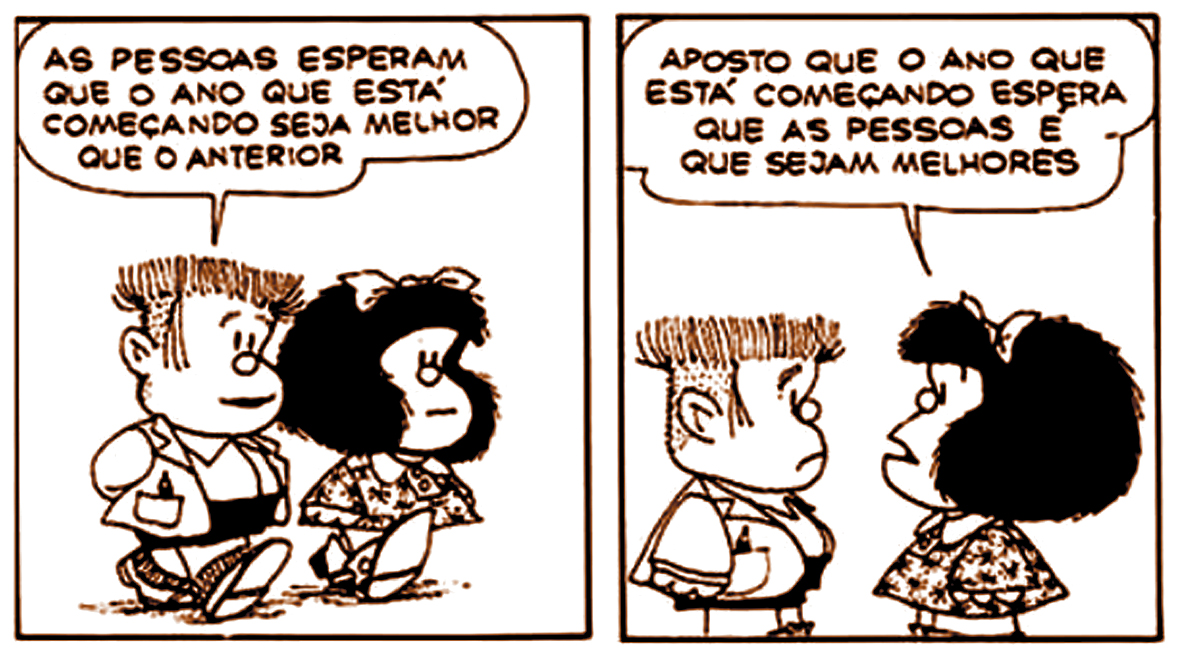
\includegraphics[width=0.75\textwidth]{figuras/mafalda}
%    \begin{flushleft}
%    \flushleft{Fonte: 
%    Elaborado pelo autor.}
%    \end{flushleft}
%    \label{fig:mafalda}
%}
%\end{figure}


%Exemplo de uso de tabela no Latex (Tabela~\ref{tab:tabelaModelo}). Ver página %72 do Manual de Normalização de Trabalhos Acadêmicos do IFCE.
%\begin{table}[th]
%    \centering
%    \caption{Legenda da Tabela no Topo.}
%    \label{tab:tabelaModelo}
%    \begin{tabular}{llll}
%    & Nota mínima & Nota máxima & Nota média\\\hline
%    Ciências Humanas (CH)     & 324,8       & 862,1       & 546,5\\
%    Ciências da Natureza (CN) & 330,6       & 876,4       & 482,2\\
%    Linguagens e Códigos (LC) & 306,2       & 814,2       & 507,9\\
%    Matemática (MT)           & 318,5       & 973,6       & 473,5\\ \hline  
%    \end{tabular}
%    \begin{flushleft}
%    \flushleft{Fonte: 
%    Instituto Brasileiro de Geografia e Estatística - IBGE.}
%    \end{flushleft}
%\end{table}
